\documentclass[aspectratio=169,9pt]{beamer}
% \documentclass[9pt]{beamer}
\usetheme[block=fill]{ru}           % Use ru theme
\usepackage{common}


\title{Linear Cryptanalysis of \MORUS}

\author{Tomer Ashur, Maria Eichlseder, Martin M. Lauridsen, Ga\"etan Leurent, Brice Minaud, Yann Rotella, Yu Sasaki,\\ \textbf{Beno\^it Viguier}}
\date[Short Occasion]{DS Lunch Talk, June 22, 2018}

\begin{document}

% -------------------------------------------------------------
\begin{frame}
  \titlepage
\end{frame}

% -------------------------------------------------------------

% -------------------------------------------------------------
\begin{frame}{Overview}
  \setbeamertemplate{section in toc}{{\color{gray}$\blacktriangleright$}~\inserttocsection}
  \tableofcontents
\end{frame}

\section{\MORUS \& \MiniMORUS}

% -------------------------------------------------------------

% -------------------------------------------------------------
\begin{frame}{What is \MORUS?}

\begin{itemize}
  \item Authenticated encryption algorithm (Encrypt-and-MAC)
  \item Designed by Wu and Huang
  % \item 3 versions:
  %   \begin{itemize}
  %     \item \MORUS[640] with 128-bit key
  %     \item \MORUS[1280-128] with 128-bit key
  %     \item \MORUS[1280-256] with 128-bit key
  %   \end{itemize}
\end{itemize}
\begin{table}[b]
\caption{Security goals of \MORUS.}
% \label{Tbl/security}
\centering
\begin{tabular}{@{}l@{\quad}c@{\qquad}c@{}}\toprule
                        & Confidentiality (bits) & Integrity (bits) \\ \midrule
\MORUS[640-128]   & 128                    & 128              \\
\MORUS[1280-128]  & 128                    & 128              \\
\MORUS[1280-256]  & 256                    & 128              \\ \bottomrule
\end{tabular}
\end{table}

\centerline{Impose rekeying every $2^{64}$ encrypted blocks.}
\end{frame}

% -------------------------------------------------------------

% -------------------------------------------------------------
\begin{frame}{What is \MORUS?}

\MORUS state:
\begin{itemize}
  \item 5 registers of 4 words.
  \item \MORUS[640], 32-bit words $\implies$ 128-bit registers $\implies$ SSE instructions.
  \item \MORUS[1280], 64-bit words $\implies$ 256-bit registers $\implies$ AVX2 instructions.
\end{itemize}
\begin{figure}[h]
  \centering
  \resizebox{0.8\textwidth}{!}{%
  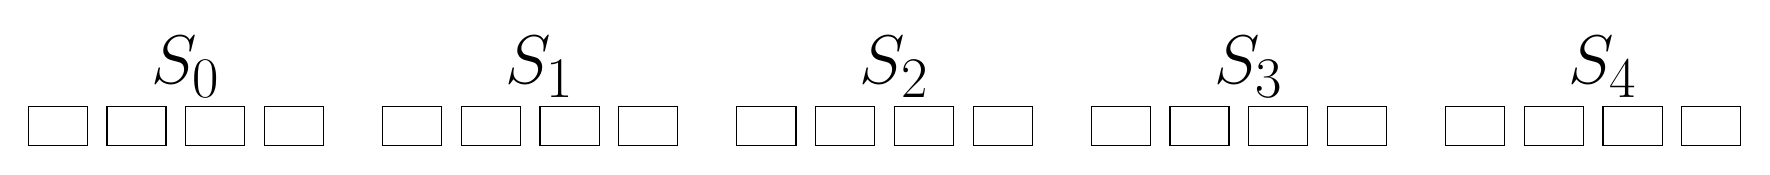
\begin{tikzpicture}[font=\Huge]

\foreach \s in {0,...,4} {
  \node (S\s) at (2+4.5*\s,1) {$S_\s$};
  \foreach \w in {0,...,3} {
    \draw (\w+4.5*\s,0) rectangle +(0.75,0.5);
  }
}

\end{tikzpicture}

  }
  % \caption{\MiniMORUS state update function.}
  % \label{fig:morus_state}
\end{figure}
\end{frame}

% -------------------------------------------------------------

% -------------------------------------------------------------
\begin{frame}{What is \MORUS?}

\begin{figure}[h]
  \substatesfalse
  \centering
  \resizebox{0.9\textwidth}{!}{%
  \begin{tikzpicture}[font=\huge]
\tikzset{oop/.style={draw, fill=none, minimum size=2ex, inner sep=0pt}}
\tikzset{oopxor/.style={oop, shape=oplus}}

\foreach \r/\t in {-4/$S^{-16}$,-3/$S^{-15}$,-1/$S^{-1}$} {
  \draw (2*\r,0) rectangle ++(0.5,3);
  \node at (0.25+2*\r,1.5) {$f$};
  \node (t-\r) at (-0.25+2*\r,3.5) {\t};
}
\foreach \r in {-4,-3} {
  \foreach \h in {0.5,1,1.5,2,2.5} {
    \draw [edge] (0.5+2*\r,\h) -- +(1.5,0);
  }
}
\foreach \h in {0.5,1,1.5,2,2.5} {
  \draw [edge] (-9,\h) -- +(1,0);
}
\node [anchor=east] at (-9,2.5) {$cst$};
\node [anchor=east] at (-9,2) {$cst$};
\node [anchor=east] at (-9,1.5) {$1^*$};
\node [anchor=east] at (-9,1) {$Key$};
\node [anchor=east] at (-9,0.5) {$Nonce$};
\node (ldots) at (0.25+2*-1.625,1.5) {\ldots\ldots};

\foreach \r in {0,1,2,3,4} {

  \draw (2*\r,0) rectangle ++(0.5,3);
  \node at (0.25+2*\r,1.5) {$f$};
  \node (t\r) at (-0.25+2*\r,3.5) {$S^\r$};
  \node (M\r) at (0.25+2*\r,-1.5) {$M^\r$};
  \node[oopxor] (xor\r) at ($(M\r) +(0,-1.5)$)  {};
  \node (C\r) at ($(M\r) +(0,-3)$) {$C^\r$};

  \draw[edge] (M\r.north) -- (0.25+2*\r,0);
  \draw[edge] (M\r.south) -- (xor\r.north);
  \draw[edge] (xor\r.south) -- (C\r.north);
}

\foreach \r in {0,1,2,3,4} {
  \foreach \h in {0.5,1,1.5,2,2.5} {
    \draw[edge] (-1.5+2*\r,\h) -- +(1.5,0);
  }
  \draw[edge] (-0.5+2*\r,2) -- +(0,-5) -- (xor\r.west);
}
\node (ldots) at (9.5,1.5) {\ldots};

\pause

\fill [ruDarkTeal,opacity=.9] (-11,-0.5) rectangle +(10,4.5);
\node at (-6,1.75) {\color{white}\textbf{RANDOM}};

\pause

\fill [black!2] (-11.1,-0.51) rectangle +(10.2,4.6);
\node [anchor=east] at (-1,2.5) {{\Large\tt rand()} $\rightarrow S_4$};
\node [anchor=east] at (-1,2) {{\Large\tt rand()} $\rightarrow S_3$};
\node [anchor=east] at (-1,1.5) {{\Large\tt rand()} $\rightarrow S_2$};
\node [anchor=east] at (-1,1) {{\Large\tt rand()} $\rightarrow S_1$};
\node [anchor=east] at (-1,0.5) {{\Large\tt rand()} $\rightarrow S_0$};


\end{tikzpicture}

  }
\end{figure}
\end{frame}

% -------------------------------------------------------------

% -------------------------------------------------------------
\begin{frame}{What is \MORUS?}

\begin{figure}[h]
  \substatesfalse
  \centering
  \resizebox{!}{0.8\textheight}{%
  \begin{tikzpicture}[xscale=1.0,yscale=1.5]

\rotwtrue
\messagetrue
\printstate

\end{tikzpicture}

  }
  % \caption{\MiniMORUS state update function.}
  % \label{fig:morus}
\end{figure}
\end{frame}

% -------------------------------------------------------------

% -------------------------------------------------------------
\begin{frame}{\MiniMORUS!}

% \begin{columns}
%   \begin{column}
\begin{figure}[h]
  \substatesfalse
  \centering
  \resizebox{!}{0.8\textheight}{%
  \begin{tikzpicture}[xscale=1.0,yscale=1.5]

\rotwfalse
\messagetrue
\printstate

\end{tikzpicture}

  }
  % \caption{\MiniMORUS state update function.}
  % \label{fig:minimorus}
\end{figure}
%   \end{column}
%   \begin{column}
%     \begin{itemize}
%       \item \MiniMORUS[640] : 32bits of security
%     \end{itemize}
%   \end{column}
% \end{columns}

\end{frame}

% -------------------------------------------------------------

% -------------------------------------------------------------
\begin{frame}{\MiniMORUS with chosen plaintext!}

\begin{figure}[h]
  \substatesfalse
  \centering
  \resizebox{!}{0.8\textheight}{%
  \begin{tikzpicture}[xscale=1.0,yscale=1.5]

\rotwfalse
\messagefalse
\printstate

\end{tikzpicture}

  }
  % \caption{\MiniMORUS state update function.}
  % \label{fig:minimorus}
\end{figure}
\end{frame}


\section{Linear Cryptanalysis of \MiniMORUS}


% -------------------------------------------------------------

% -------------------------------------------------------------
\begin{frame}{Weight and Bias}

\begin{center}
\texttt{x = u + y $\oplus$ (z $\land$ t)}\\
Can be linear approximated with\\
\texttt{E: x = u + y}
\end{center}

This linear approximation holds with a bias $\varepsilon$:
$$\Pr(E) = \frac{1}{2} + \varepsilon$$

The {\it correlation} and {\it weight} of an approximation is:
\begin{align*}
\corr(E) &\eqdef 2\Pr(E)-1 = 2 \varepsilon\\
\weight(E) &\eqdef -\log_2|\corr(E)|
\end{align*}

\begin{alertblock}{Pilling Up Lemma (Matsui M., 1993)}
  The correlation (resp. weight) of an XOR of independent variables is equal to
  the product (resp. sum) of their individual correlations (resp. weights)
\end{alertblock}

\end{frame}

% -------------------------------------------------------------

% -------------------------------------------------------------
\begin{frame}{\MiniMORUS : trails $\alpha, \beta, \gamma, \delta, \varepsilon$}

  \begin{figure}
    \substatesfalse
    \rotwfalse
    \statesfalse
    \messagefalse

    \resizebox{!}{0.78\textheight}{%
    \begin{tikzpicture}[xscale=0.65,yscale=1.5]%{{{
  \rotwfalse
  \messagefalse
  \printstate
  \draw[trail, alpha]
    (C) -- node[right] {$i$} (lll-1)
    (lll-1) -- (tlll-1) (lll-1) -- (xor-1) (xor-1) -- (xnd-1)
    (xnd-1) -- (and-1) (xor-1) -- (txor-1) (txor-1) -- (tanB0) (tanB0) -- (tanB0-|and0.east)
    (and0) -- (xnd0) (xnd0) -- (tlll-1) (xnd0) -- (xor0)
    (and-1.east|-tanA-1) -- (tanA-1) (tanA-1) -- (txor0) (txor0) -- (xor0)
    (xor0) -- (lll0) (lll0) -- (W40) node[below] {$i+b_0$}
    ;
  \draw[trail, alpha, dashed]
    (and-1.east|-tanB-1) -- (tanB-1) (tanB-1) -- (tanA0) (tanA0) -- (tanA0-|and0.east);
  % \draw[alpha, very thick] (W40) + (0,-0.2) ellipse (0.6cm and 0.175cm);

  \draw (W42) + (0,-0.5) node[below] {weight($\alpha^t_i$) = 1 (not 2)};

\end{tikzpicture}%}}}

    }
    \resizebox{!}{0.78\textheight}{%
    \begin{tikzpicture}[xscale=0.65,yscale=1.5]%{{{
  \rotwfalse
  \messagefalse
  \printstate
  \draw[trail, beta]
    (C) -- node[right] {$i$} (lll-1)
    (lll-1) -- (tlll-1) (lll-1) -- (xor-1) (xor-1) -- (xnd-1)
    (tlll-1) -- (W-20) node[above] {$i$}
    (xor-1) -- (txor-1) (txor-1) -- (W-21) node[above] {$i$}
    (xnd-1) -- (and-1)
    (W40) node[below] {\phantom{$i$}};

    \draw (W42) + (0,-0.5) node[below] {weight($\beta^t_i$) = 1};
    % \draw[beta, very thick] (W-21) + (0,+0.175) ellipse (0.2cm and 0.15cm);

\end{tikzpicture}%}}}

    }
    \resizebox{!}{0.78\textheight}{%
    \begin{tikzpicture}[xscale=0.65,yscale=1.5]%{{{
  \rotwfalse
  \messagefalse
  \printstate
  \draw[trail, gamma]
    (W-21) node[above] {$i$} -- (xnd1) (xnd1) -- (xor1) (xor1) -- (lll1)
    (xnd1) -- (and1)
    (xor1) -- (txor1)
    (txor1) -- (W-24) node[above] {$i$}
    (lll1) -- (W41) node[below] {$i+b_1$}
    ;
    % \draw[gamma,very thick] (W-24) + (0,+0.175) ellipse (0.2cm and 0.15cm);
    \draw (W42) + (0,-0.5) node[below] {weight($\gamma^t_i$) = 1};

\end{tikzpicture}%}}}

    }
    \resizebox{!}{0.78\textheight}{%
    \begin{tikzpicture}[xscale=0.65,yscale=1.5]%{{{
  \rotwfalse
  \messagefalse
  \printstate
  \draw[trail, delta]
    (W-24) node[above] {$i$} -- (xnd4) (xnd4) -- (xor4) (xnd4) -- (and4)
    (xor4) -- (lll4) (xor4) -- (txor4) (txor4) -- (W42) node[below] {$i$}
    (lll4) -- (W44) node[below] {$i+b_4$}
    ;

    % \draw[delta, very thick] (W42) + (0,-0.175) ellipse (0.2cm and 0.15cm);
    \draw (W42) + (0,-0.5) node[below] {weight($\delta^t_i$) = 1};

\end{tikzpicture}%}}}

    }
    \resizebox{!}{0.78\textheight}{%
    \begin{tikzpicture}[xscale=0.65,yscale=1.5]%{{{
  \rotwfalse
  \messagefalse
  \printstate
  \draw[trail, epsil]
    (W-22) node[above] {$i$} -- (xnd2) (xnd2) -- (xor2) (xnd2) -- (and2)
    (xor2) -- (lll2) (xor2) -- (txor2) (txor2) -- (W40) node[below] {$i$}
    (lll2) -- (W42) node[below] {$i+b_2$}
    ;

  \draw (W42) + (0,-0.5) node[below] {weight($\varepsilon^t_i$) = 1};
\end{tikzpicture}%}}}

    }
  \end{figure}

\end{frame}


% -------------------------------------------------------------

% -------------------------------------------------------------

\begin{frame}{Building Trails}

\begin{figure}
  \includegraphics[width=0.9\textwidth]{lego.jpg}
\end{figure}

\end{frame}

% -------------------------------------------------------------

% -------------------------------------------------------------
\begin{frame}{\MiniMORUS[640] : Building trails with $\chi_1$ and $\chi_2$}

  \begin{figure}
    \resizebox{!}{0.90\textheight}{%
      \newcommand{\M}[2]{1.65,-1.5*#1-.25-.25*#2}
\newcommand{\C}[1]{-.1,-.25-1.5*#1}
\renewcommand{\S}[2]{.25+.25*#2,-1.5*#1}

% \begin{tikzpicture}[xscale=3, yscale=1.5, every node/.style={font=\scriptsize,inner sep=2pt}]
\begin{tikzpicture}[xscale=3, yscale=1.5, every node/.style={font=\scriptsize,inner sep=2pt}]
  % \begin{scope}
    \foreach \r in {0,...,3} { \draw[gray, rounded corners=2pt] (0,-\r*1.5) rectangle ++(1.5,-1.5); }
    \foreach \r in {0,...,4} { \draw (\S{0}{\r}) node[above] {$S_{\r}$}; }
    \draw (\C{0}|-\S{0}{0}) node[above] {$C$};

    \draw[beta, thick]  (\C{1}) node[above left] {0} -| (\S{1}{0}) node[below right] {0}
                 (\C{1}-|\S{1}{0}) -| ([xshift=-1pt]\S{1}{1}) node[above] {0\,}
                 (\M{1}{0}) node[right] {$\beta_0$};

    \pause
    \draw[alpha, thick] (\C{0}) node[left] {27} -| (\S{1}{0}) node[above right] {0}
                 (\M{0}{0}) node[right] {$\alpha_{27}$};


     \pause
     \draw[gamma, thick] (\S{1}{1}) node[above] {\,0} -- (\S{2}{1}) node[above left] {31\!\!}
                  (\S{1}{1}) ++(0,-.75) -| ([xshift=-1pt]\S{1}{4}) node[above] {0\,}
                  (\M{1}{2}) node[right] {$\gamma_0$};

    \pause

    \draw[beta, thick]  (\C{2}) node[above left] {31} -| ([xshift=-1pt]\S{2}{0}) node[below left] {31\!}
                 (\C{2}) -| (\S{2}{1}) node[below left] {31\!\!}
                 (\M{2}{0}) node[right] {$\beta_{31,}$};

    % \pause

    \draw[alpha, thick] ([yshift=-3.0pt]\C{1}) node[below left] {26} -| ([xshift=-1pt]\S{2}{0}) node[above left] {31\!}
                (\M{1}{1}) node[right] {$\alpha_{26,}$};

    \pause

    \draw[delta, thick] (\S{1}{4}) node[above] {\,0} -- (\S{2}{4}) node[above right] {13}
                 (\S{1}{4}) ++(0,-1.25) -| ([xshift=2pt]\S{2}{2}) node[below] {0} node[black] {$\times$}
                 (\M{1}{3}) node[right] {$\delta_0$};

    \pause

    \draw[gamma, thick] ([xshift=2pt]\S{2}{1}) node[below right] {13} -- ([xshift=2pt]\S{3}{1}) node[above right] {12}
                 ([xshift=2pt]\S{2}{1}) ++(0,-.75) -| (\S{2}{4}) node[below right] {13}
                 (\M{2}{2}) node[right] {$\gamma_{13}$};

    % \pause

    \draw[beta, thick]  ([yshift=-1.5pt]\C{2}) node[left] {13} -| (\S{2}{0}) node[below right] {\!\!13}
                 ([yshift=-1.5pt]\C{2}-|\S{2}{0}) -| ([xshift=1pt]\S{2}{1}) node[above] {\,\,\,13};
    \draw[beta, thick]  (\M{2}{0}) + (0.11,-0.02) node[right] {$_{, 13}$};

    % \pause

    \draw[alpha, thick] ([yshift=-1.5pt]\C{1}) node[left] {8} -| (\S{2}{0}) node[above right] {\!\!13}
                 (\M{1}{1}) + (0.12,0) node[right] {$_{, 8}$};

    % \pause

    \draw[beta, thick]  (\C{3}) node[left] {12} -| (\S{3}{0}) node[below right] {12}
                 (\C{3}-|\S{3}{0}) -| ([xshift=2pt]\S{3}{1}) node[below right] {12}
                 (\M{3}{0}) node[right] {$\beta_{12}$};

    % \pause

    \draw[alpha, thick] ([yshift=-3.0pt]\C{2}) node[below left] {7} -| (\S{3}{0}) node[above right] {12}
                 (\M{2}{1}) node[right] {$\alpha_7$};

    \pause
    \draw (\S{4}{2}) node[above] {\large  $\chi_1$: {\it estimated} weight 11};

    \draw (\S{4}{1}) + (0,-0.25) node [below] {\large $C^0_{27} \oplus C^1_{0} \oplus C^1_{8} \oplus C^1_{26} \oplus C^2_{7} \oplus C^2_{13} \oplus C^2_{31} \oplus C^3_{12} \to S^2_{2,0}$};

  \pause

  \begin{scope}[xshift=2.5cm]
    \foreach \r in {1,...,4} { \draw[gray, rounded corners=2pt] (0,-\r*1.5) rectangle ++(1.5,-1.5); }
    \foreach \r in {0,...,4} { \draw (\S{1}{\r}) node[above] {$S_{\r}$}; }
    \draw (\C{0}|-\S{1}{0}) node[above] {$C$};

    \draw[epsil, thick] (\S{2}{2}) node[above] {0} node[black] {$\times$} -- (\S{3}{2}) node[below] {7\,}
                 (\S{2}{2}) ++(0,-1.00) -| ([xshift=-4pt]\S{3}{0}) node[above left] {0}
                 (\M{2}{3}) node[right] {$\varepsilon_0$};
    \pause

    \draw[delta, thick] (\S{2}{4}) node[above] {\,7} -- (\S{3}{4}) node[above right] {20}
                 (\S{2}{4}) ++(0,-1.25) -| ([xshift=1pt]\S{3}{2}) node[below] {\,7}
                 (\M{2}{4}) node[right] {$\delta_7$};

    \pause

    \draw[gamma, thick] (\S{2}{1}) node[above] {\,7} -- (\S{3}{1}) node[above left] {6\!}
                 (\S{2}{1}) ++(0,-.75) -| ([xshift=-1pt]\S{2}{4}) node[above] {7\,}
                 (\M{2}{2}) node[right] {$\gamma_7$};

    \draw[gamma, thick] ([xshift=2pt]\S{3}{1}) node[below right] {20} -- ([xshift=2pt]\S{4}{1}) node[above right] {19}
                 ([xshift=2pt]\S{3}{1}) ++(0,-.75) -| (\S{3}{4}) node[below right] {20}
                 (\M{3}{2}) node[right] {$\gamma_{20}$};

    \pause

    \draw[beta, thick]  (\C{2}) node[above left] {7} -| (\S{2}{0}) node[below right] {7}
                (\C{2}-|\S{2}{0}) -| ([xshift=-1pt]\S{2}{1}) node[above] {7\,}
                (\M{2}{0}) node[right] {$\beta_7$};

    \draw[beta, thick]  (\C{3}) node[above left] {6} -| ([xshift=-1pt]\S{3}{0}) node[below left] {6\!}
                 ([xshift=-1pt]\C{3}-|\S{3}{0}) -| (\S{3}{1}) node[below left] {6\!}
                 (\M{3}{0}) node[right] {$\beta_{20,6}$};
    \draw[beta, thick]  ([yshift=-1.5pt]\C{3}) node[left] {20} -| (\S{3}{0}) node[below right] {\!20}
                 ([yshift=-1.5pt]\C{3}-|\S{3}{0}) -| ([xshift=1pt]\S{3}{1}) node[above] {\,\,\,\,20};

    \draw[beta, thick]  (\C{4}) node[left] {19} -| (\S{4}{0}) node[below right] {19}
                (\C{4}-|\S{4}{0}) -| ([xshift=2pt]\S{4}{1}) node[below right] {19}
                (\M{4}{0}) node[right] {$\beta_{19}$};

    \pause

    \draw[alpha, thick] (\C{1}) node[left] {2} -| (\S{2}{0}) node[above right] {7}
                 (\M{1}{0}) node[right] {$\alpha_{2}$};

    \draw[alpha, thick] ([yshift=-1.5pt]\C{2}) node[left] {15} -| (\S{3}{0}) node[above right] {\!20}
                 (\M{2}{1}) node[right] {$\alpha_{15,1,27}$};
    \draw[alpha, thick] ([yshift=-3.0pt]\C{2}) node[below left] {1} -| ([xshift=-1pt]\S{3}{0}) node[above left] {6\!};
    \draw[alpha, thick] ([yshift=-4.5pt]\C{2}) node[below] {\,\,\,\,27} -| ([xshift=-3pt]\S{3}{0}) node[below] {0\,\,};

    \draw[alpha, thick] ([yshift=-3.0pt]\C{3}) node[below left] {14} -| (\S{4}{0}) node[above right] {19}
                 (\M{3}{1}) node[right] {$\alpha_{14}$};

    \draw (\S{5}{2}) node[above] {\large $\chi_2$: {\it estimated} weight 13};

    \draw (\S{1}{4}) + (0,0.5)  node [above] {\large $C^1_{2} \oplus C^2_{1} \oplus C^2_{7} \oplus C^2_{15} \oplus C^2_{27} \oplus C^3_{6} \oplus C^3_{14} \oplus C^3_{20} \oplus C^4_{19} \to  S^2_{2,0}$};
    % \draw (\S{5}{2}) node[above] {\normalsize $\chi_2$: weight 9 (not 13)};
    % \draw (\S{0}{2}) node[below] {\normalsize \MiniMORUS[640]};
  \end{scope}
\end{tikzpicture}

    }
  \end{figure}

\end{frame}


% -------------------------------------------------------------

% -------------------------------------------------------------
\begin{frame}{\MiniMORUS : Weight of $\beta^t_i \oplus \gamma^t_i$}

\begin{columns}
\begin{column}{0.6\textwidth}
  \begin{figure}
    \resizebox{!}{0.90\textheight}{%
      \begin{tikzpicture}[xscale=0.75,yscale=1.5]
  \rotwfalse
  \messagefalse
  \statesfalse
  \printstate

  \draw[trail, beta]
    (C) -- node[right] {$i$} (lll-1)
    (lll-1) -- (tlll-1) (lll-1) -- (xor-1) (xor-1) -- (xnd-1)
    (tlll-1) -- (W-20) node[above] {$i$}
    (xor-1) -- (txor-1) %(txor-1) -- (W-21) node[above] {$i$}
    %(xnd-1) -- (and-1)
    (W40) node[below] {\phantom{$i$}}
    ;
  \draw[trail, gamma]
    %(W-21) node[above] {$i$}
    (txor-1) -- (xnd1)
    (xnd1) -- (xor1) (xor1) -- (lll1)
    %(xnd1) -- (and1)
    (xor1) -- (txor1)
    (txor1) -- (W-24) node[above] {$i$}
    (lll1) -- (W41) node[below] {$i+b_1$}
    ;
  % \draw[trail, beta,  dotted] (and-1) -- (and-1-|and1);
  % \draw[trail, gamma, dotted] (and1)  -- (and-1-|and1) node[above, black] {=};
  \node (eq) at ($(and-1|-and1)+(-1,-2.4pt)$) {=};
  % \node ()
  \node [opand,fill=beta] at (and-1) {$\cdot$};
  \node [opand,fill=gamma] at (and1) {$\cdot$};
  \draw[beta,{Circle[sep=-1.8pt]}-]  ($(and-1)+(0,-2.4pt)$) -| (eq);
  \draw[gamma,{Circle[sep=-1.8pt]}-] ($(and1)+(0,-2.4pt)$) -- (eq);
\end{tikzpicture}

    }
  \end{figure}
\end{column}
\begin{column}{0.3\textwidth}  %%<--- here
        Weight of $\beta^t_i \oplus \gamma^t_i$ is 0 (not 2).
  \end{column}
\end{columns}
\end{frame}

% -------------------------------------------------------------

% -------------------------------------------------------------
\begin{frame}{\MiniMORUS[640] : Weight corrected}

  \begin{figure}
    \resizebox{!}{0.90\textheight}{%
      \input{tikz/trails-nopause.tex}
    }
  \end{figure}

\end{frame}


% -------------------------------------------------------------

% -------------------------------------------------------------
\begin{frame}{\MiniMORUS : Full Trail}

\begin{itemize}
  \item \MiniMORUS[640]
  $$\chi_1 \oplus \chi_2 = C^0_{27} \oplus C^1_{0} \oplus C^1_{2} \oplus C^1_{8} \oplus C^1_{26} \oplus C^2_{1} \oplus C^2_{13} \oplus C^2_{15} \oplus
   C^2_{27} \oplus C^2_{31} \oplus C^3_{6} \oplus C^3_{12} \oplus C^3_{14} \oplus C^3_{20} \oplus C^4_{19} \to 0$$
   \item \MiniMORUS[1280]
  $$C^0_{51} \oplus C^1_{0} \oplus C^1_{25} \oplus C^1_{33} \oplus C^1_{55} \oplus C^2_{4} \oplus C^2_{7} \oplus C^2_{29} \oplus C^2_{37} \oplus
  C^2_{38} \oplus C^2_{46} \oplus C^2_{51} \oplus C^3_{11} \oplus C^3_{20} \oplus C^3_{42} \oplus C^3_{50} \oplus C^4_{24} \to 0$$
\end{itemize}

  In both case, the weight of the trail is 7 + 9 = 16.

\end{frame}

% -------------------------------------------------------------

% -------------------------------------------------------------
\begin{frame}{\MiniMORUS : Experimental verification}

  \begin{table}[h!]
    % \caption{Experimental verification of trail correlations.}
    % \label{tab:miniapproximations}
    \centerline{
    \begin{tabular}{@{}llSSS@{}}
      % \toprule
      & & \multicolumn{3}{@{}c@{}}{Weight} \\
      \cmidrule{3-5}
      \multicolumn{2}{@{}l}{Approximations for \MiniMORUS[640]}
               & {Exp.} & {Bool.} & {Meas.} \\
      \midrule
      $\chi_1$ & $S^{2,2}_0 = C^0_{27} \oplus C^1_{0, 8, 26} \oplus C^2_{7,13,31} \oplus C^3_{12}$
               & 7    & 7     & 7 \\
      $\chi_2$ & $S^{2,2}_0 = C^1_{2} \oplus C^2_{1,7,15,27} \oplus C^3_{6,14,20} \oplus C^4_{19}$
               & 9    & 9     & 9 \\
      $\chi$   & $0 = C^0_{27} \oplus C^1_{0, 2, 26, 8} \oplus C^2_{1,13,15,27,31} \oplus C^3_{6,12,14,20} \oplus C^4_{19}$
               & 16   & 16    & 15.5 \\
      \midrule
      \multicolumn{2}{@{}l}{Approximations for \MiniMORUS[1280]} \\
      \midrule
      $\chi_1$ & $S^{2,2}_0 = C^0_{51} \oplus C^1_{0, 33, 55} \oplus C^2_{4,37,46} \oplus C^3_{50}$
               & 7    & 7     & 7 \\
      $\chi_2$ & $S^{2,2}_0 = C^1_{25} \oplus C^2_{7,29,38,51} \oplus C^3_{11,20,42} \oplus C^4_{24}$
               & 9    & 9     & 9 \\
      $\chi$   & $0 = C^0_{51} \oplus C^1_{0, 25, 33, 55} \oplus C^2_{4,7,29,37,38,46,51} \oplus C^3_{11,20,42,50} \oplus C^4_{24}$
               & 16   & 16    & 15.9 \\
      \bottomrule
    \end{tabular}
    }
  \end{table}

  \begin{center}
    The programs we used to verify the bias experimentally are available at:\\
    \centerline{\url{https://github.com/ildyria/MorusBias}}
  \end{center}

\end{frame}

\section{Extension to \MORUS and Consequences}

% -------------------------------------------------------------

% -------------------------------------------------------------
\begin{frame}{From \MiniMORUS to \MORUS}

\begin{itemize}
  \itemsep1.5em
  \item Trail extension:\\
    $S_{i,j}$ in \MiniMORUS is translated into $S_{i,j} \oplus S_{i,j + w} \oplus S_{i,j + 2w} \oplus S_{i,j + 3w}$ in \MORUS\\
    e.g. $S_{2,0}$ in \MiniMORUS[1280] $\iff S_{2,0} \oplus S_{2,64} \oplus S_{2,128} \oplus S_{2,192}$ in \MORUS[1280].
   \item Weight implication:\\
     word ``\textit{equality}'' occurs with probability $\frac{1}{2^4}$ $\implies$ weight $\times 4$\\

    \item $\beta_i + \gamma_i$ has weight 0 in \MiniMORUS but weight 4 in \MORUS\\
\end{itemize}

\begin{alertblock}{Weight of the trails}
  \centering
  \MORUS[640]: Weight($\chi$) = 73\\
  \MORUS[1280]: Weight($\chi$) = 76
\end{alertblock}

\end{frame}


% -------------------------------------------------------------

% -------------------------------------------------------------
\begin{frame}{Impact for \MORUS}

\begin{itemize}
  \item \textbf{Keystream correlation}
    \begin{itemize}
      \item The bias is \textit{absolute}: does not depends on Key or Nounce!
      \item Similar to RC4, BEAST attack\ldots
      \item Known plaintext $\implies$ Distinguisher.
      \item Multiple fixed plaintext $\implies$ plaintext recovery.
    \end{itemize}
  \pause
  \item \textbf{Data complexity}
    \begin{itemize}
      \item Immune to rekeying every $2^{64}$ encrypted block.
      \item Require $2^{146}$ blocks for \MORUS[640]
      \item Require $2^{152}$ blocks for \MORUS[1280] \textbf{\alert{(violate 256-bit confidentiality claim)}}
      \item trail is immune to bit-shift:\\
        - save $2^5$ data for \MORUS[640].\\
        - save $2^6$ data for \MORUS[1280].\\
      \item Not practical. :(
    \end{itemize}
\end{itemize}

\end{frame}

% -------------------------------------------------------------

% -------------------------------------------------------------
\begin{frame}[standout]

\centerline{\huge\textbf{\url{https://eprint.iacr.org/2018/464.pdf}}}

\end{frame}


\end{document}
